\section{Hyperparameter Optimization}

\begin{frame}{Hyperparameter Optimization}
    思想:超参数的选择多种多样,如何高效地找到最优超参数?

    几种算法
    \begin{itemize}
        \item Bayesian Optimization
        \item Gradient Optimization
        \item Random Search
        \item Multi-armed Bandit: Successive Halving (SH) Algorithm
        \item Neural Architecture Search (NAS): ProxylessNAS
    \end{itemize}
\end{frame}

\begin{frame}{Bayesian Optimization \& Gradient Optimization \& Random Search}
    \begin{itemize}
        \item 人工智能回答的非常好
        \item 看看课件基本上了解大致原理就行
    \end{itemize}
\end{frame}

\begin{frame}{Multi-armed Bandit: Successive Halving (SH) Algorithm}
    算法:
    \begin{center}
        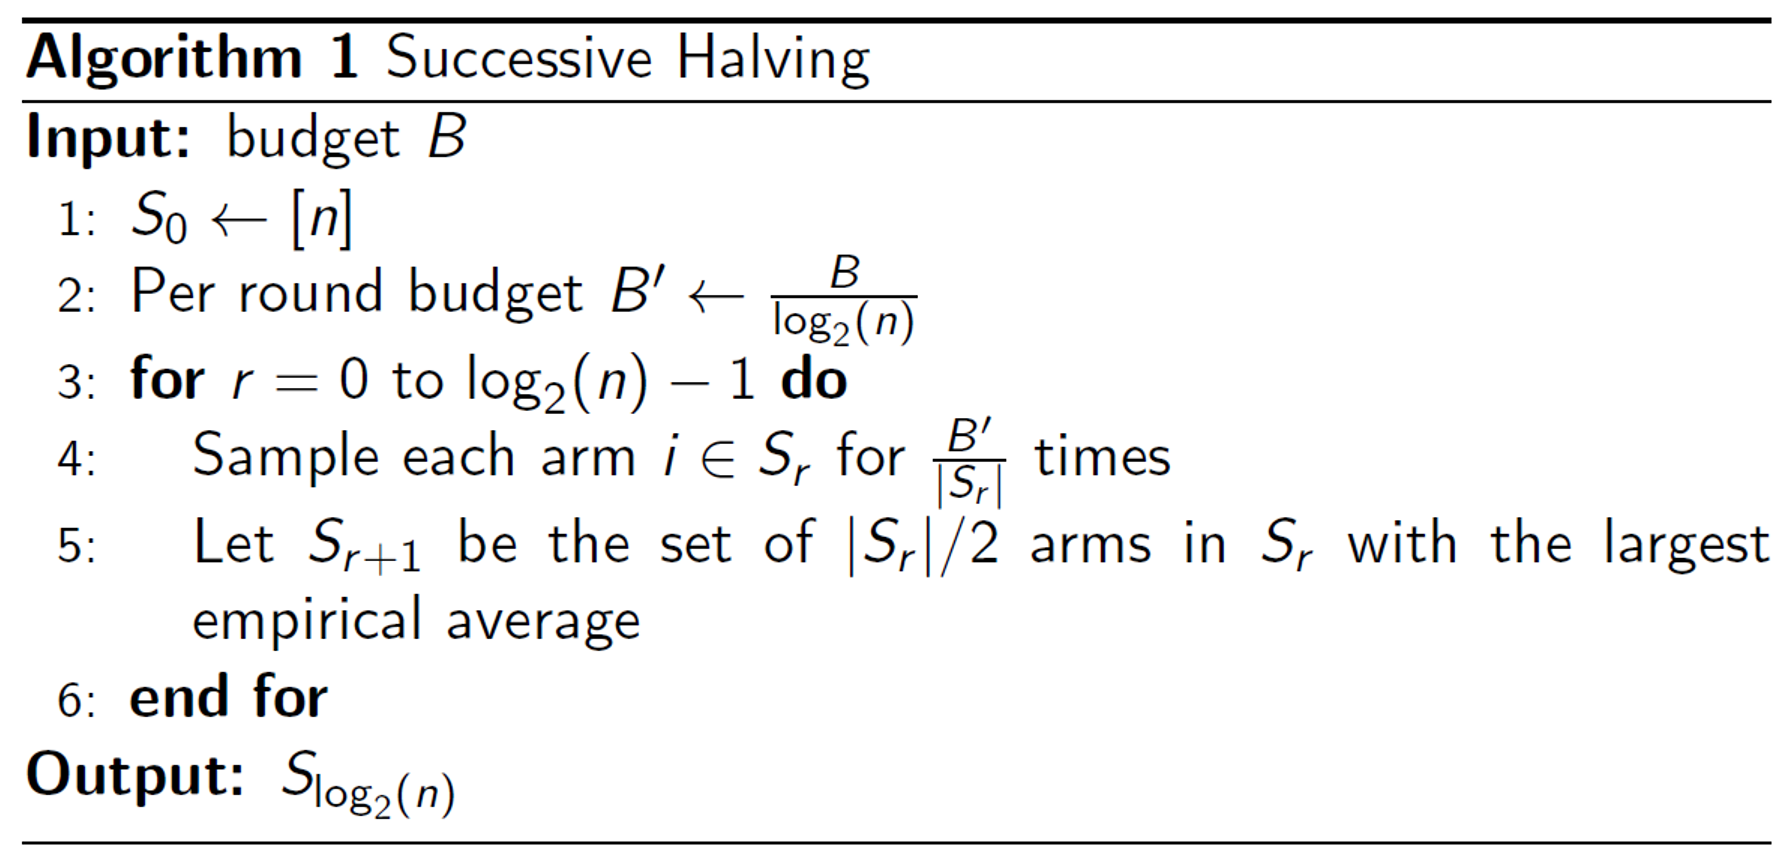
\includegraphics[width=0.6\textwidth]{assets/sh.png}
    \end{center}
\end{frame}

\begin{frame}{SH Algorithm Analysis}
    \begin{block}{Theorem}
        不妨假设$v_1 \geqslant v_2 \geqslant \cdots \geqslant v_n$,记 $\Delta_i = v_1 - v_i$。

        在取摇老虎机次数 $B = O\left( H_2 \log n \log \frac{\log n}{\delta} \right) $时,上述算法以至少 $1 - \delta$ 的概率找到了最优的老虎机,其中 $H_2 =\max_{i > 1} \frac{i}{\Delta_i^{2}}$。
    \end{block}
    证明思路:
    \begin{itemize}
        \item 每一个 iteration 中最优的老虎机被淘汰的概率被 bound 住
        \item 通过 union bound 证明最后最优的老虎机被淘汰的概率也被 bound 住
    \end{itemize}
\end{frame}

\begin{frame}{SH Algorithm in Hyperparameter Optimization}
    算法:
    \begin{center}
        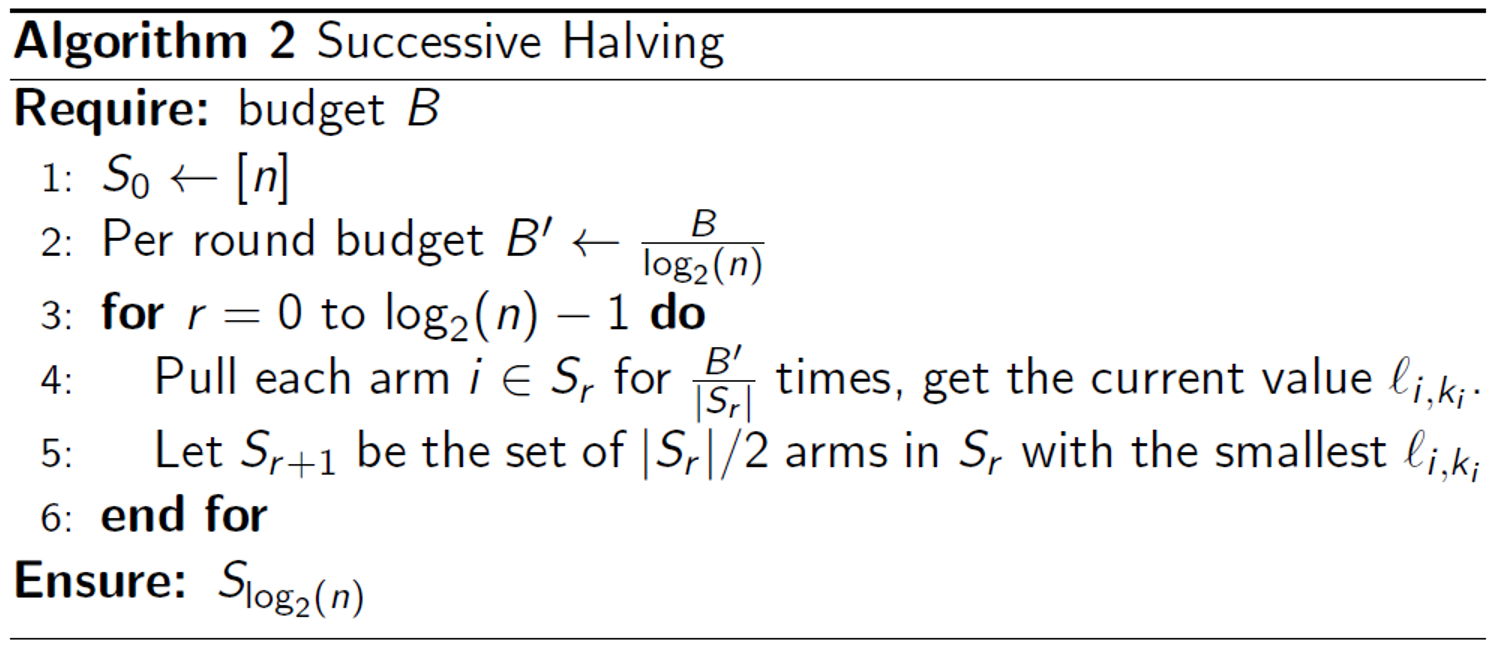
\includegraphics[width=0.6\textwidth]{assets/sh2.png}
    \end{center}
    \begin{itemize}
        \item 由于 Hyperparameter Optimization 问题与原始老虎机问题不同:老虎机中是每次玩老虎机,每次可以获得一个独立的输出;但 Hyperparameter Optimization 中每次训练模型,是时间累计的,故要进行一定的修改。
        \item 这也有一个理论保证,详见课件。
    \end{itemize}
\end{frame}

\begin{frame}{Neural Architecture Search: ProxylessNAS}
    \begin{center}
        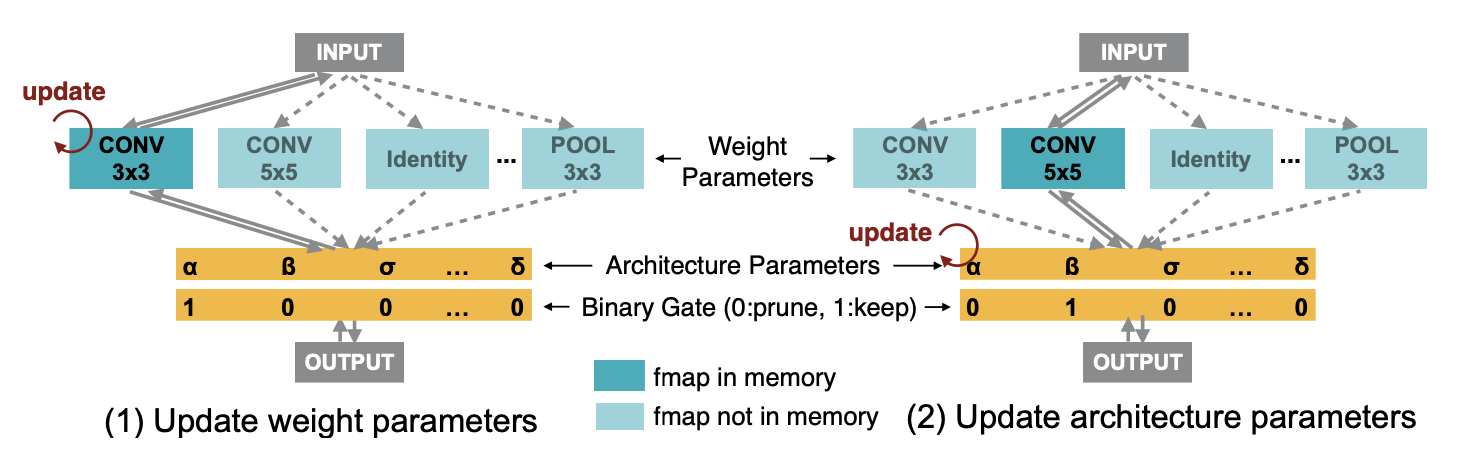
\includegraphics[width=0.6\textwidth]{assets/plnas.png}
    \end{center}
    \begin{itemize}
        \item 先构建由很多组成部分和连接方式的参数数量极大的模型,其中有一些特殊的层,对应的参数称为 architecture parameter,其他正常的模型参数称为 weight parameter。
        \item 训练方法:交替训练。先固定 architecture parameter,训练 weight parameter(训练方式与通常模型一样);再固定 weight parameter,训练 architecture parameter,学习最好的 architecture。
        \item architecture parameter更新时由于有采样部分,无法梯度更新,只能近似: $\frac{\partial L}{\partial \alpha_i} = \sum_{j=1}^{N} \frac{\partial L}{\partial p_j}\frac{\partial p_j}{\partial \alpha_i} \approx \sum_{j=1}^{N} \frac{\partial L}{\partial g_j}\frac{\partial p_j}{\partial \alpha_i}$
    \end{itemize}
\end{frame}
